\documentclass[]{article}
\usepackage{lmodern}
\usepackage{amssymb,amsmath}
\usepackage{ifxetex,ifluatex}
\usepackage{fixltx2e} % provides \textsubscript
\ifnum 0\ifxetex 1\fi\ifluatex 1\fi=0 % if pdftex
  \usepackage[T1]{fontenc}
  \usepackage[utf8]{inputenc}
\else % if luatex or xelatex
  \ifxetex
    \usepackage{mathspec}
  \else
    \usepackage{fontspec}
  \fi
  \defaultfontfeatures{Ligatures=TeX,Scale=MatchLowercase}
    \setmainfont[]{Arial Nova}
\fi
% use upquote if available, for straight quotes in verbatim environments
\IfFileExists{upquote.sty}{\usepackage{upquote}}{}
% use microtype if available
\IfFileExists{microtype.sty}{%
\usepackage{microtype}
\UseMicrotypeSet[protrusion]{basicmath} % disable protrusion for tt fonts
}{}
\usepackage[margin=1in]{geometry}
\usepackage{hyperref}
\hypersetup{unicode=true,
            pdfauthor={Ben Cole - s3412349},
            pdfborder={0 0 0},
            breaklinks=true}
\urlstyle{same}  % don't use monospace font for urls
\usepackage{graphicx,grffile}
\makeatletter
\def\maxwidth{\ifdim\Gin@nat@width>\linewidth\linewidth\else\Gin@nat@width\fi}
\def\maxheight{\ifdim\Gin@nat@height>\textheight\textheight\else\Gin@nat@height\fi}
\makeatother
% Scale images if necessary, so that they will not overflow the page
% margins by default, and it is still possible to overwrite the defaults
% using explicit options in \includegraphics[width, height, ...]{}
\setkeys{Gin}{width=\maxwidth,height=\maxheight,keepaspectratio}
\IfFileExists{parskip.sty}{%
\usepackage{parskip}
}{% else
\setlength{\parindent}{0pt}
\setlength{\parskip}{6pt plus 2pt minus 1pt}
}
\setlength{\emergencystretch}{3em}  % prevent overfull lines
\providecommand{\tightlist}{%
  \setlength{\itemsep}{0pt}\setlength{\parskip}{0pt}}
\setcounter{secnumdepth}{5}
% Redefines (sub)paragraphs to behave more like sections
\ifx\paragraph\undefined\else
\let\oldparagraph\paragraph
\renewcommand{\paragraph}[1]{\oldparagraph{#1}\mbox{}}
\fi
\ifx\subparagraph\undefined\else
\let\oldsubparagraph\subparagraph
\renewcommand{\subparagraph}[1]{\oldsubparagraph{#1}\mbox{}}
\fi

%%% Use protect on footnotes to avoid problems with footnotes in titles
\let\rmarkdownfootnote\footnote%
\def\footnote{\protect\rmarkdownfootnote}

%%% Change title format to be more compact
\usepackage{titling}

% Create subtitle command for use in maketitle
\providecommand{\subtitle}[1]{
  \posttitle{
    \begin{center}\large#1\end{center}
    }
}

\setlength{\droptitle}{-2em}

  \title{Assessing the Probability of the St.~Louis Blues\\
Winning the Stanley Cup}
    \pretitle{\vspace{\droptitle}\centering\huge}
  \posttitle{\par}
  \subtitle{Three Simulations based on Constant Elo Team
Ratings\\[2\baselineskip]MATH2223 - Sports Analytics\\
Course Project}
  \author{Ben Cole - s3412349}
    \preauthor{\centering\large\emph}
  \postauthor{\par}
      \predate{\centering\large\emph}
  \postdate{\par}
    \date{Print Date: 29/06/2019}

\usepackage{booktabs}
\usepackage{longtable}
\usepackage{array}
\usepackage{multirow}
\usepackage{wrapfig}
\usepackage{float}
\usepackage{colortbl}
\usepackage{pdflscape}
\usepackage{tabu}
\usepackage{threeparttable}
\usepackage{threeparttablex}
\usepackage[normalem]{ulem}
\usepackage{makecell}
\usepackage{xcolor}

\begin{document}
\maketitle

{
\setcounter{tocdepth}{3}
\tableofcontents
}
\section{Abstract}\label{abstract}

\section{Introduction}\label{introduction}

The National Hockey League (hereon NHL) is the North American ice hockey
competition held each year across the winter months of the Northern
hemisphere. The regular season begins in October and usually ends in
April the following year, with the finals playoffs series culminating in
the competition for the coveted Stanley Cup usually in June. (NHL, 2019)

\subsection{St.~Louis Blues -
Underdogs}\label{st.louis-blues---underdogs}

The St.~Louis Blues were the winners of the 2018-2019 Stanley Cup
playoffs, winning a 4-3 series against the Boston Bruins. The Blues
winning the Stanley Cup was paticularly extraordinary not only because
it was the first in their history as a club in the NHL, but also because
they faced off against the Bruins have appeared so regularly in the
Stanley Cup Playoffs. Since joining the NHL in 1967, the St Louis Blues
have contested the Stanley Cup Playoffs only 4 times, whilst the Boston
Bruins have made it to the Cup Playoffs 10 times since 1967 (and a total
20 since joining the NHL in 1924). (NHL, 2019)

What arguably made the St.~Louis Blues appearance in the Stanley Cup
Finals most incredible was that they ranked last in January of the same
season. Sometime between January and April they managed to claw their
way to clinching a playoffs appearance. (Bardown, 2019)

\subsection{NHL Season and Post-Season
Structure}\label{nhl-season-and-post-season-structure}

The NHL contained a total of 31 teams in the 2019 season. These 31 teams
were split across two conferences, Eastern and Western. Each conference
comprised two divisions each; Metropolitan and Atlantic in the Eastern
Conference and Central and Pacific in the Western Conference. (NHL,
2019)

Throughout the regular season each team will play 82 games, which are a
mixture of home and away fixtures. As the playing season is
approximately 27 weeks, these 82 games average out to be more than three
games per week. Therefore, unlike many Australian sporting codes, there
are no ``rounds'' in the NHL but simply game numbers. Further, there is
no structure or restriction to which game each team is playing. For
example, one team may be playing their 26th game against an opponent
that is playing their 23rd. (NHL, 2019)\\
If a team wins a game in the regular season they are awarded 2 points
for the win. If the game has a tied scoreline at the end of the third
20-minute period it will go into overtime. If the scoreline is still
tied at the end of two overtime periods then a shootout is played until
a winner is decided. The team that wins by any method, including
overtime or shootout, is still awarded 2 points. The team that loses in
overtime or shootout is awarded one point. If the game is decided before
overtime the losing team will be awarded 0 points. (MacDonald, R, 2018)

\begin{table}[t]

\caption{\label{tab:unnamed-chunk-2}Points awarded for different win types in NHL regular season}
\centering
\begin{tabular}{l|r|r}
\hline
Win Type & Winning Team Points & Losing Team Points\\
\hline
Not Overtime & 2 & 0\\
\hline
Overtime or Shootout & 2 & 1\\
\hline
\end{tabular}
\end{table}

Once the regular season has finished and team standings have been
calculated a bracketed finals system is drawn up for the playoffs. The
finals playoffs follow a repeating knockout structure that has 3 rounds
before reaching the Stanley Cup playoffs. Each conference follows the
same structure, so only one will be described as follows:

\subsubsection{Playoffs Selection}\label{playoffs-selection}

A total of 16 teams from both conferences qualify for the finals
playoffs. The top three teams in each division are awarded spots in the
playoffs. As there are two divisions in each conference, this results in
6 teams in each conference making it to the finals. A further two spots
are awarded to the next two highest ranking teams in the conference that
did not make the playoffs. As this is based on standings in the
conference overall, it's possible for a division to send two wildcards
through to the playoffs.

\paragraph{First Round}\label{first-round}

In the first round the highest-ranked division winner plays the
lowest-ranked wildcard entrant. The lesser-ranked division winner then
plays the remaining wildcard entrant. Teams ranked second and third
within each division play each other. Each pairing is decided by a
series of games which is decided when one team wins 4 times. This
results in a series length that can be anywhere between 4 (winning 4-0)
and 7 (winning 4-3), or the best of 7 games.

\paragraph{Second Round}\label{second-round}

The winners of each of each First Round series then play each other in
the second round, keeping within divisions and ignoring wildcards.
Again, a best of 7 series is played in each pairing.

\paragraph{Conference Round}\label{conference-round}

The winners of each Second Round series face off in the Conference
round, which decides the winner of each conference via a best of 7 games
series.

\paragraph{Stanley Cup}\label{stanley-cup}

The winners of each Conference Round series play off in the Stanley Cup
finals, which are also a best of 7 series.

\begin{figure}
\centering
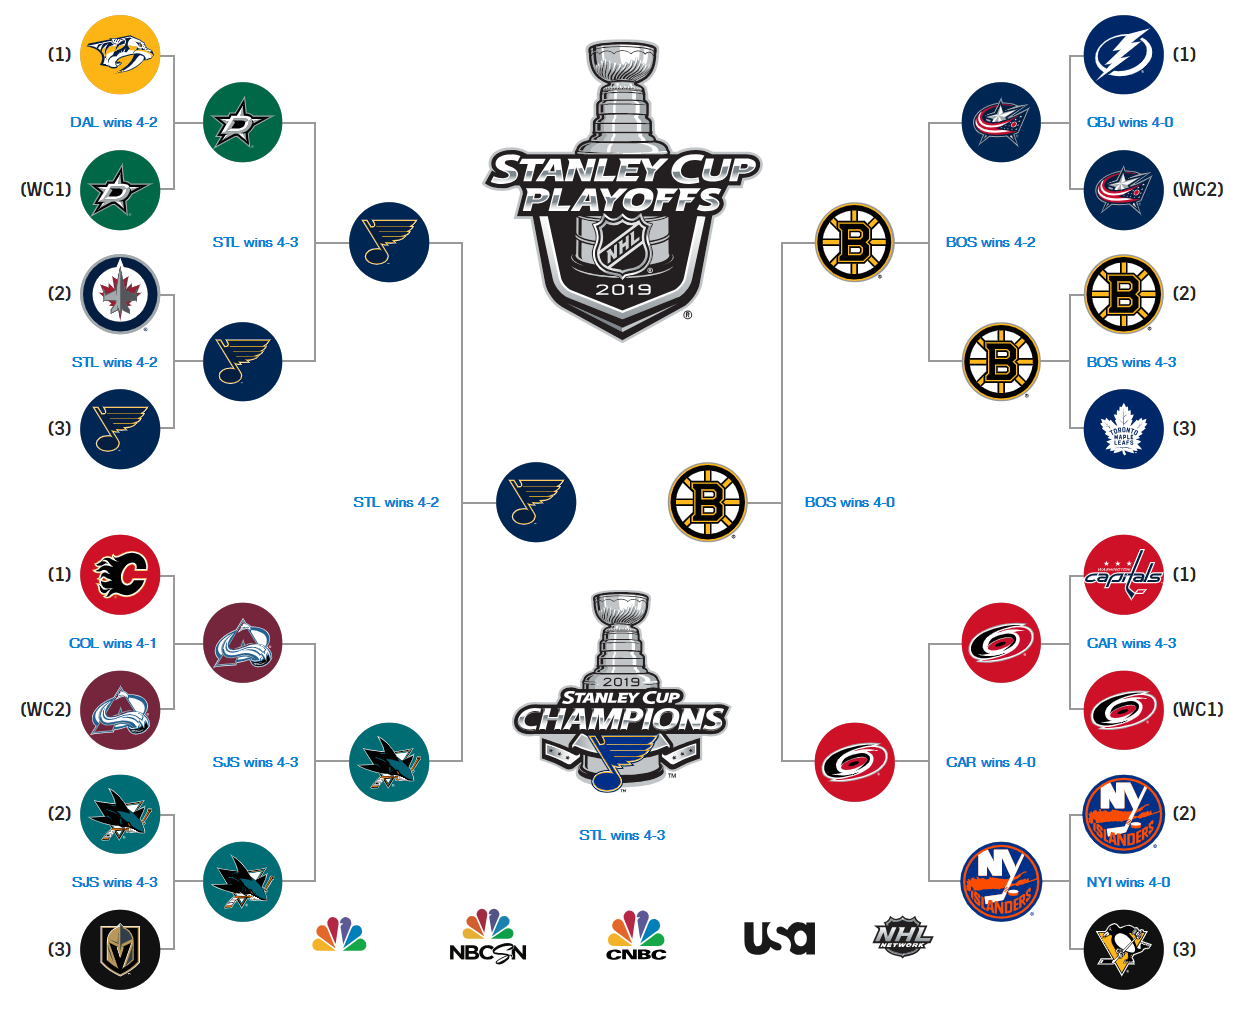
\includegraphics{Finals_2019.png}
\caption{As it happened: The 2018-2019 Finals Playoffs Series \nSource:
\url{https://www.nhl.com/stanley-cup-playoffs}}
\end{figure}

\section{Aims}\label{aims}

Considering the turn around in the St.~Louis Blues' performance within
the season and the

\section{Literature Review}\label{literature-review}

\section{Methods}\label{methods}

\section{Results}\label{results}

\section{Discussion}\label{discussion}

\subsection{Limitations}\label{limitations}

\section{Conclusions}\label{conclusions}

\section{References}\label{references}

National Hockey League, 2019, \emph{Stanley Cup® Playoffs}, NHL, viewed
23 June 2019, \url{https://www.nhl.com/stanley-cup-playoffs}

National Hockey League, 2019, \emph{Standings - 2018-2019}, NHL, viewed
29 June 2019, \url{https://www.nhl.com/standings/2018/division}

National Hockey League, 2019, \emph{Stanley Cup Playoffs format,
qualification system}, NHL, viewed 24 June 2019,
\url{https://www.nhl.com/news/stanley-cup-playoffs-format-qualification-system/c-711015}

National Hockey League, 2019, \emph{All-Time Stanley Cup Champions},
NHL, viewed 29 June 2019,
\url{https://www.nhl.com/info/all-time-stanley-cup-winners}

MacDonald, R, 2018, \emph{Fixing the NHL Points System and Re-Seeding
the 2018 Stanley Cup Playoffs}, Last Word on Hockey,
\url{https://lastwordonhockey.com/2018/04/11/fixing-the-nhl-points-system-and-re-seeding-the-2018-playoffs/}

Bardown, 2019, \emph{With post-season clinched, the St.~Louis Blues make
NHL history with incredible turnaround}, Bardown, Viewed 29 June 2019,
\url{https://www.bardown.com/the-st-louis-blues-make-nhl-history-with-incredible-turnaround-1.1282314}


\end{document}
